% Copyright 2007 by Till Tantau
%
% This file may be distributed and/or modified
%
% 1. under the LaTeX Project Public License and/or
% 2. under the GNU Public License.
%
% See the file doc/licenses/LICENSE for more details.


\lecture[24]{Using linear regression}{lecture-text}

\subtitle{confidence intervals, outliers, and leverage}

\date{1 December 2015}

% pp. 505-527


\begin{document}

\begin{frame}
  \maketitle
\end{frame}


\begin{frame}\frametitle<presentation>{Outline}
  \tableofcontents
\end{frame}


\section{The linear model}

%%%% %%%%%%% %%%%%%%
\section{Interpretation}


%%%%%%
\begin{frame}{Residuals}

  \ldots are what's left over, $e_i$:
  \begin{align*}
    \hat y_i &= b_0 + b_1 x_i \\
    e_i &= y_i - \hat y_i
  \end{align*}

  \begin{center}
    \includegraphics<1>{loblolly-age-height}
    \includegraphics<2>{loblolly-resids}
  \end{center}

  \vspace{1em}
  \alert{What does this mean?}

\end{frame}


%%%%%%
\begin{frame}{Nonlinearity}

    \begin{center}
    \includegraphics<1>{nonlinear1.pdf}
    \includegraphics<2>{nonlinear2.pdf}
    \end{center}

    If the true relationship isn't linear, \\
    then linear regression might not be the right tool.
    \pause

    \alert{But it might be a good first pass.}


\end{frame}




\section{Diagnostic plots}


%%%%%%
\begin{frame}{Residuals versus predicted}
    Checks for nonlinearity; \uncover<3->{heteroskedasticity (different variances)}
    \begin{center}
        \includegraphics<1>{nonlinear2-resids.pdf}
        \includegraphics<2>[width=\textwidth]{usc-temps-fit-resid.pdf}
        \includegraphics<3>{hetersked-resids.pdf}
    \end{center}

    \structure{The hope} is to see \alert{no structure} in the residual plot.

\end{frame}


% 
% %%%%%%
% \begin{frame}{What can go wrong?}
% 
%     \begin{center}
%         \includegraphics[width=\textwidth]<1>{many-regressions-1.pdf}
%         \includegraphics[width=\textwidth]<2>{many-regressions-2.pdf}
%         \includegraphics[width=\textwidth]<3>{many-regressions-3.pdf}
%     \end{center}
% 
% \end{frame}



\begin{frame}{Common errors: nonindependence}


  \alert{ Observations are dependent: } \\

  20 measurements of serum cholesterol ($X$) and glucose ($Y$) \ldots \\
  10 from each patient.
  \vspace{2em}

      \structure{Example:} 
      \begin{center}
        \includegraphics<1>[width=\textwidth]{nonindep-0}
        \includegraphics<2>[width=\textwidth]{nonindep}
      \end{center}

\end{frame}


\begin{frame}{Common errors: misinterpretation}
    
  $r$ estimates the \alert{population correlation} $\rho$ \\
  \structure{only}
  under the bivariate random sampling model.

  \vspace{2em}


      \structure{Example:} 
      \begin{center}
        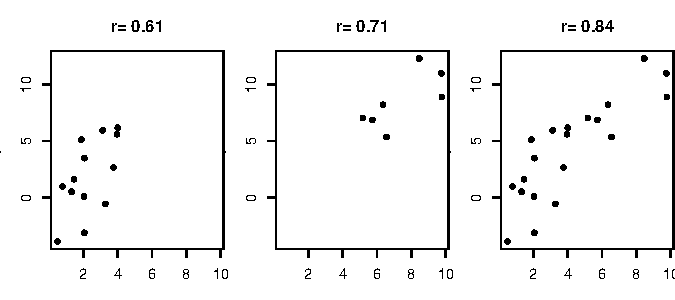
\includegraphics[width=\textwidth]{r-interp}
      \end{center}


\end{frame}

\begin{frame}{Example: Loblolly}
  Heights and ages of 84 Loblolly pines, \alert{$r=0.99$}:
  \begin{center}
    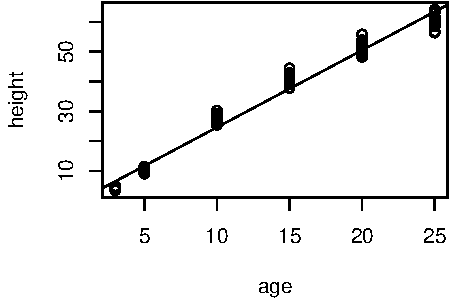
\includegraphics{loblolly-age-height}
  \end{center}

  \vspace{1em}
  
  What's wrong with this:

  ``Tree age explains 98\% of the variance of Loblolly pine height in the forest.''

\end{frame}



%%%%%%
\begin{frame}{Outliers}

    An \alert{outlier} is a data point unusually far from the rest (in some sense; usually in the sense of having \alert{large residuals}).
    \begin{center}
        \includegraphics<1>[width=3in]{fig-12-6-3.png}
        \includegraphics<2>[width=2in]{fig-12-6-3.png}
    \end{center}
    \pause

    These usually indicate deviations from the model;\\
    and may have a large effect on the results.


    \vspace{2em}

    \structure{What to do:} investigate, use robust statistics.

\end{frame}


%%%%%%
\begin{frame}{Leverage points}

    A \alert{leverage point} is one that \emph{could} have a large effect on the regression.
    (i.e.\ moving it changes the slope of the regression line a lot)
    \begin{center}
        \includegraphics<1>[width=3in]{fig-12-6-3.png}
        \includegraphics<2>[width=2in]{fig-12-6-3.png}
    \end{center}
    \pause

    \vspace{1em}

    These are \structure{far from the center of mass}.


    \vspace{1em}

    \structure{What to do:} investigate.

\end{frame}



%%%%%%
\begin{frame}{Influential points}

    An \alert{influential point} is one that actually \alert{is} affecting the regression line a lot -- if it was removed, the slope would change dramatically.
    \begin{center}
        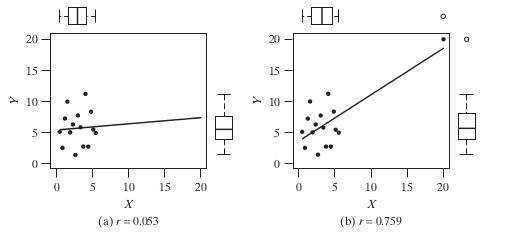
\includegraphics[width=3in]{fig-12-6-4.png}
    \end{center}

    \vspace{2em}

    \structure{What to do:} investigate.

\end{frame}


\section<article>{Summary}
\section<presentation>*{Summary}

\begin{frame}{Summary}
  \begin{enumerate}
      \item Linear regression fits a model where the mean of $Y$ is a linear function of $X$
      \item and the variances do not depend on $X$.
      \item Under the ``random subsampling model'',
      \item $b_0$ and $b_1$ are good estimates of the terms in the linear relationship
      \item and $s_e$ is a good estimate of the residual SD.
      \item Testing for correlation is equivalent to testing for $b_1=0$,
      \item which we can do with a $t$ test and $\SE_{b_1}$.
      \item Look at the data to check if the conditions are met.
  \end{enumerate}
\end{frame}

% homework
\begin{frame}{Homework}
  \begin{center}

      Two 8.5"$\times$11" pages, two-sided, of handwritten notes.

    \vspace{2em}

    Bring a calculator (besides your phone).

  \end{center}
\end{frame}


\end{document}





